% ---------------------------------------------------------------------------
\section{Data Sources and Synthetic Contextual Generation}
\label{sec:data}
% ---------------------------------------------------------------------------

\subsection{The analytical base}

The labelled base is the Kaggle competition sample \emph{House Prices: Advanced
Regression Techniques}, which contains 1,460 residential transactions in Ames, Iowa
completed between 2006 and 2010, described by 79 explanatory attributes and the
realised sale price \citep{kaggle2016,decock2011}. A further 1,459 transactions are
supplied without a price. The platform never observes a sale price at listing time,
so the unlabelled file is the analogue of a live listing stream and is used for
scoring only, never for fitting.

The target is heavily right-skewed. The median sale price is 163,000 \USD{} and the
mean 180,933 \USD, with a skewness of 1.881 that falls to 0.122 after a natural
logarithm. The sample spans 25 neighbourhoods and a wide range of construction
vintages, quality grades and lot sizes, and it contains the usual assessor-coded
categorical variables in which a missing value often means that a feature is absent
rather than unknown. These properties drive three later decisions: the log target
(Section~\ref{sec:features}), the absence-to-``None'' cleaning rule
(Section~\ref{sec:cleaning}) and the use of conformal rather than Gaussian intervals
(Section~\ref{sec:models}).

\subsection{Why contextual data had to be generated}

The competition attributes describe the property, not the market in which it is
listed. A real platform also observes distances to schools, hospitals and transit,
the quality of the surrounding neighbourhood, renovation history, how long comparable
listings take to sell, and macro-financial conditions at the moment of listing. None
of these are present in the base file, and all are plausibly relevant to price. The
project therefore generates 21 contextual fields, each documented in a data
dictionary stating its type, unit, valid range, generation logic and the business
assumption behind it.

The announcement suggests the Faker library for this task \citep{faker2026}. The team
instead used NumPy generators with explicit distributions, because the fields
required here are quantitative context rather than synthetic identities, and because
a fixed seed with documented parametric distributions makes the realism argument
auditable in a way that free-form fake data does not. The generator is deterministic
given seed 42 and the input row order, which is what allows every number in this
report to be reproduced.

\subsection{Generation logic and realism}

Table~\ref{tab:synthetic} summarises the five families of generated fields. The
common principle is that a documented neighbourhood tier, an expert prior about
sub-market desirability in Ames, drives the mean of each distribution, while
dispersion and idiosyncratic noise are supplied by the random component. The tier is
a prior about location, not an estimate derived from the sale price, and this is the
central leakage control of the generation step.

\begin{table}[htbp]
\centering
\caption{The five families of synthetic contextual fields, with representative
generation logic and the sanity check used to assess realism. All 21 fields are
documented individually in the data dictionary (Appendix~\ref{app:dictionary}).}
\label{tab:synthetic}
\small
\begin{tabularx}{\linewidth}{@{}L{0.14\linewidth}L{0.255\linewidth}L{0.33\linewidth}X@{}}
\toprule
\textbf{Family} & \textbf{Representative fields} & \textbf{Generation mechanism} & \textbf{Realism check} \\
\midrule
Location and amenity access & \f{neigh\_lat}, \f{neigh\_lon}, four distances, \f{park\_area\_ha}, \f{amenity\_density\_1\_5km} & Centroid plus Gaussian jitter; log-normal distances whose medians decline with the tier & Distances inside plausible city bounds \\
Neighbourhood quality & \f{school\_rating}, \f{walk\_score}, \f{crime\_index}, \f{amenity\_score} & Clipped Gaussian draws around tier means; amenity score is a weighted composite rescaled to 0--100 & Mean amenity score rises from 43.5 in tier 1 to 85.5 in tier 5 \\
Renovation history & \f{renovation\_flag}, \f{renovation\_scope} & Derived from assessor construction and remodelling years; scope by remodelling lag & Shares consistent with base data; no price enters the rule \\
Marketing duration & \f{days\_on\_market}, \f{listing\_date} & Log-normal draw with tier, quality, month, rate and supply effects; clipped to 1--365 days & Median 31 days, 90th percentile 69 days \\
Macro-financial context & \f{mortgage\_rate\_pct}, \f{hpi\_index}, \f{hpi\_yoy\_pct}, \f{months\_supply}, \f{local\_unemployment\_pct} & Monthly paths interpolated between documented anchors with AR(1) noise & Rate range 4.67--6.78\%; index falls from 100 to a trough of 93.69 \\
\bottomrule
\end{tabularx}
\end{table}

The macro block deserves particular attention because it later drives the monitoring
alerts. Its anchors reproduce the shape of the 2006--2011 United States housing
cycle: mortgage rates near 6.5 per cent in 2006, falling through 2008 and 2009 to
about 5.0 per cent; a price index that peaks around 2007 and declines to a trough in
2009; and months of supply peaking at 8.8 in 2009 before easing.
Figure~\ref{fig:macro} confirms that interpolation plus AR(1) noise produces smooth,
plausible monthly paths rather than independent random draws.

\begin{figure}[htbp]
\centering
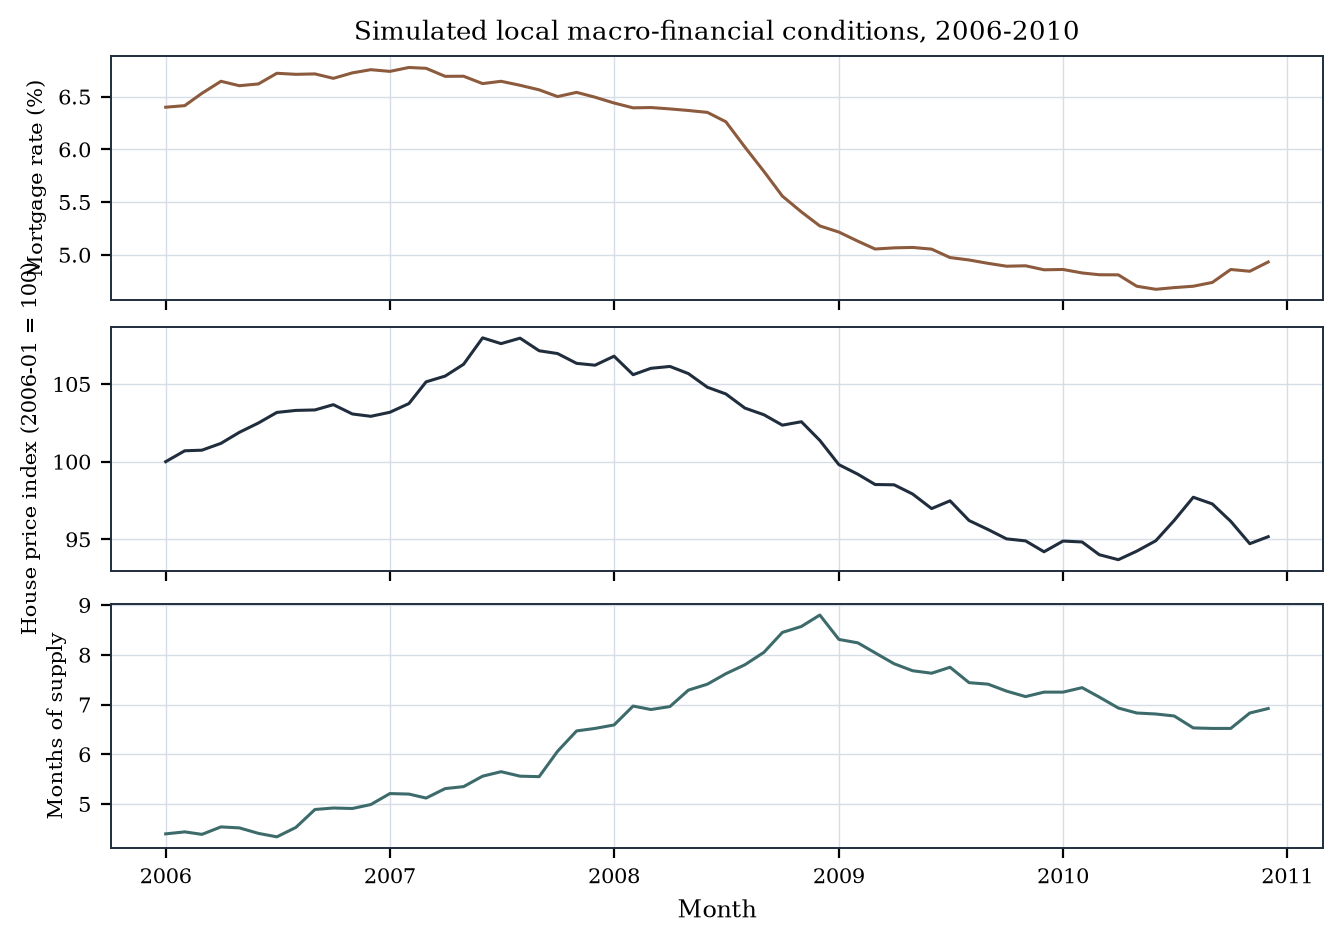
\includegraphics[width=0.74\linewidth]{fig12_macro_trends.png}
\caption{Simulated macro-financial conditions, 2006--2010: the 30-year mortgage rate,
the local house price index (January 2006 = 100) and months of supply. The anchors
reproduce the shape of the United States housing cycle; monthly AR(1) noise prevents
the series from looking mechanically interpolated.}
\label{fig:macro}
\end{figure}

Three pieces of evidence support the realism of the generated context. First,
internal consistency: the amenity score averages 43.5 in tier-1 neighbourhoods, 53.1
in tier 2, 63.0 in tier 3, 73.8 in tier 4 and 85.5 in tier 5, so the measure
separates sub-markets in the direction local knowledge predicts without having been
fitted to prices. Second, external consistency: the generated fields correlate with
price in the expected directions, with crime at $-0.55$, distance to transit at
$-0.37$, distance to school at $-0.28$ and the amenity score at $0.615$ in Pearson
terms and $0.652$ in Spearman terms. Third, behavioural plausibility: marketing
duration has a median of 31 days and a 90th percentile of 69 days, and it lengthens
for weaker locations, lower-quality properties, winter listings and high-interest-rate
periods, which is the pattern platforms actually observe.

The argument has a limit, revisited in Section~\ref{sec:recommendations}. Because
the generator encodes assumptions, the coefficient on a synthetic field measures the
assumption as much as the market. A strong amenity coefficient is evidence that the
model recovered the simulated gradient, not that a one-point improvement raises the
price of a specific house by a specific amount. Causal language is therefore avoided,
and the synthetic fields are treated as controls that improve conditional accuracy
rather than as policy levers.

\subsection{Leakage controls}

Target leakage is the most common way for a housing model to report a flattering and
worthless result. Three controls are enforced. The generator never reads the sale
price; variables recorded after the transaction closes (sale condition, sale type,
days on market, listing date, sale year and month) are excluded from the model even
though they are present in the analytical table; and the neighbourhood tier is not
supplied as an input, so the model must infer sub-market effects from observed
location and amenity fields. The exclusion list is maintained in configuration and
exercised by the test suite, so a change that reintroduces a leaking column fails a
test rather than silently inflating accuracy.
